
\documentclass[8pt]{article}

\usepackage[utf8]{inputenc}

\usepackage{amsmath, bm}
\usepackage{graphicx}
\usepackage{amssymb}
\usepackage{float}
\usepackage{caption}
\usepackage{subcaption}
% set font size to 11pt

% set margin
\usepackage[margin=0.5in]{geometry}


\begin{document}

% insert pdf cover page here

\title{Lab report: 3A3 Supersonic Nozzle}
\author{lwp26}
\date{October 2023}
\maketitle

\section{Part 1 Convergent - divergent nozzle}

\begin{figure}[H]
    \centering
    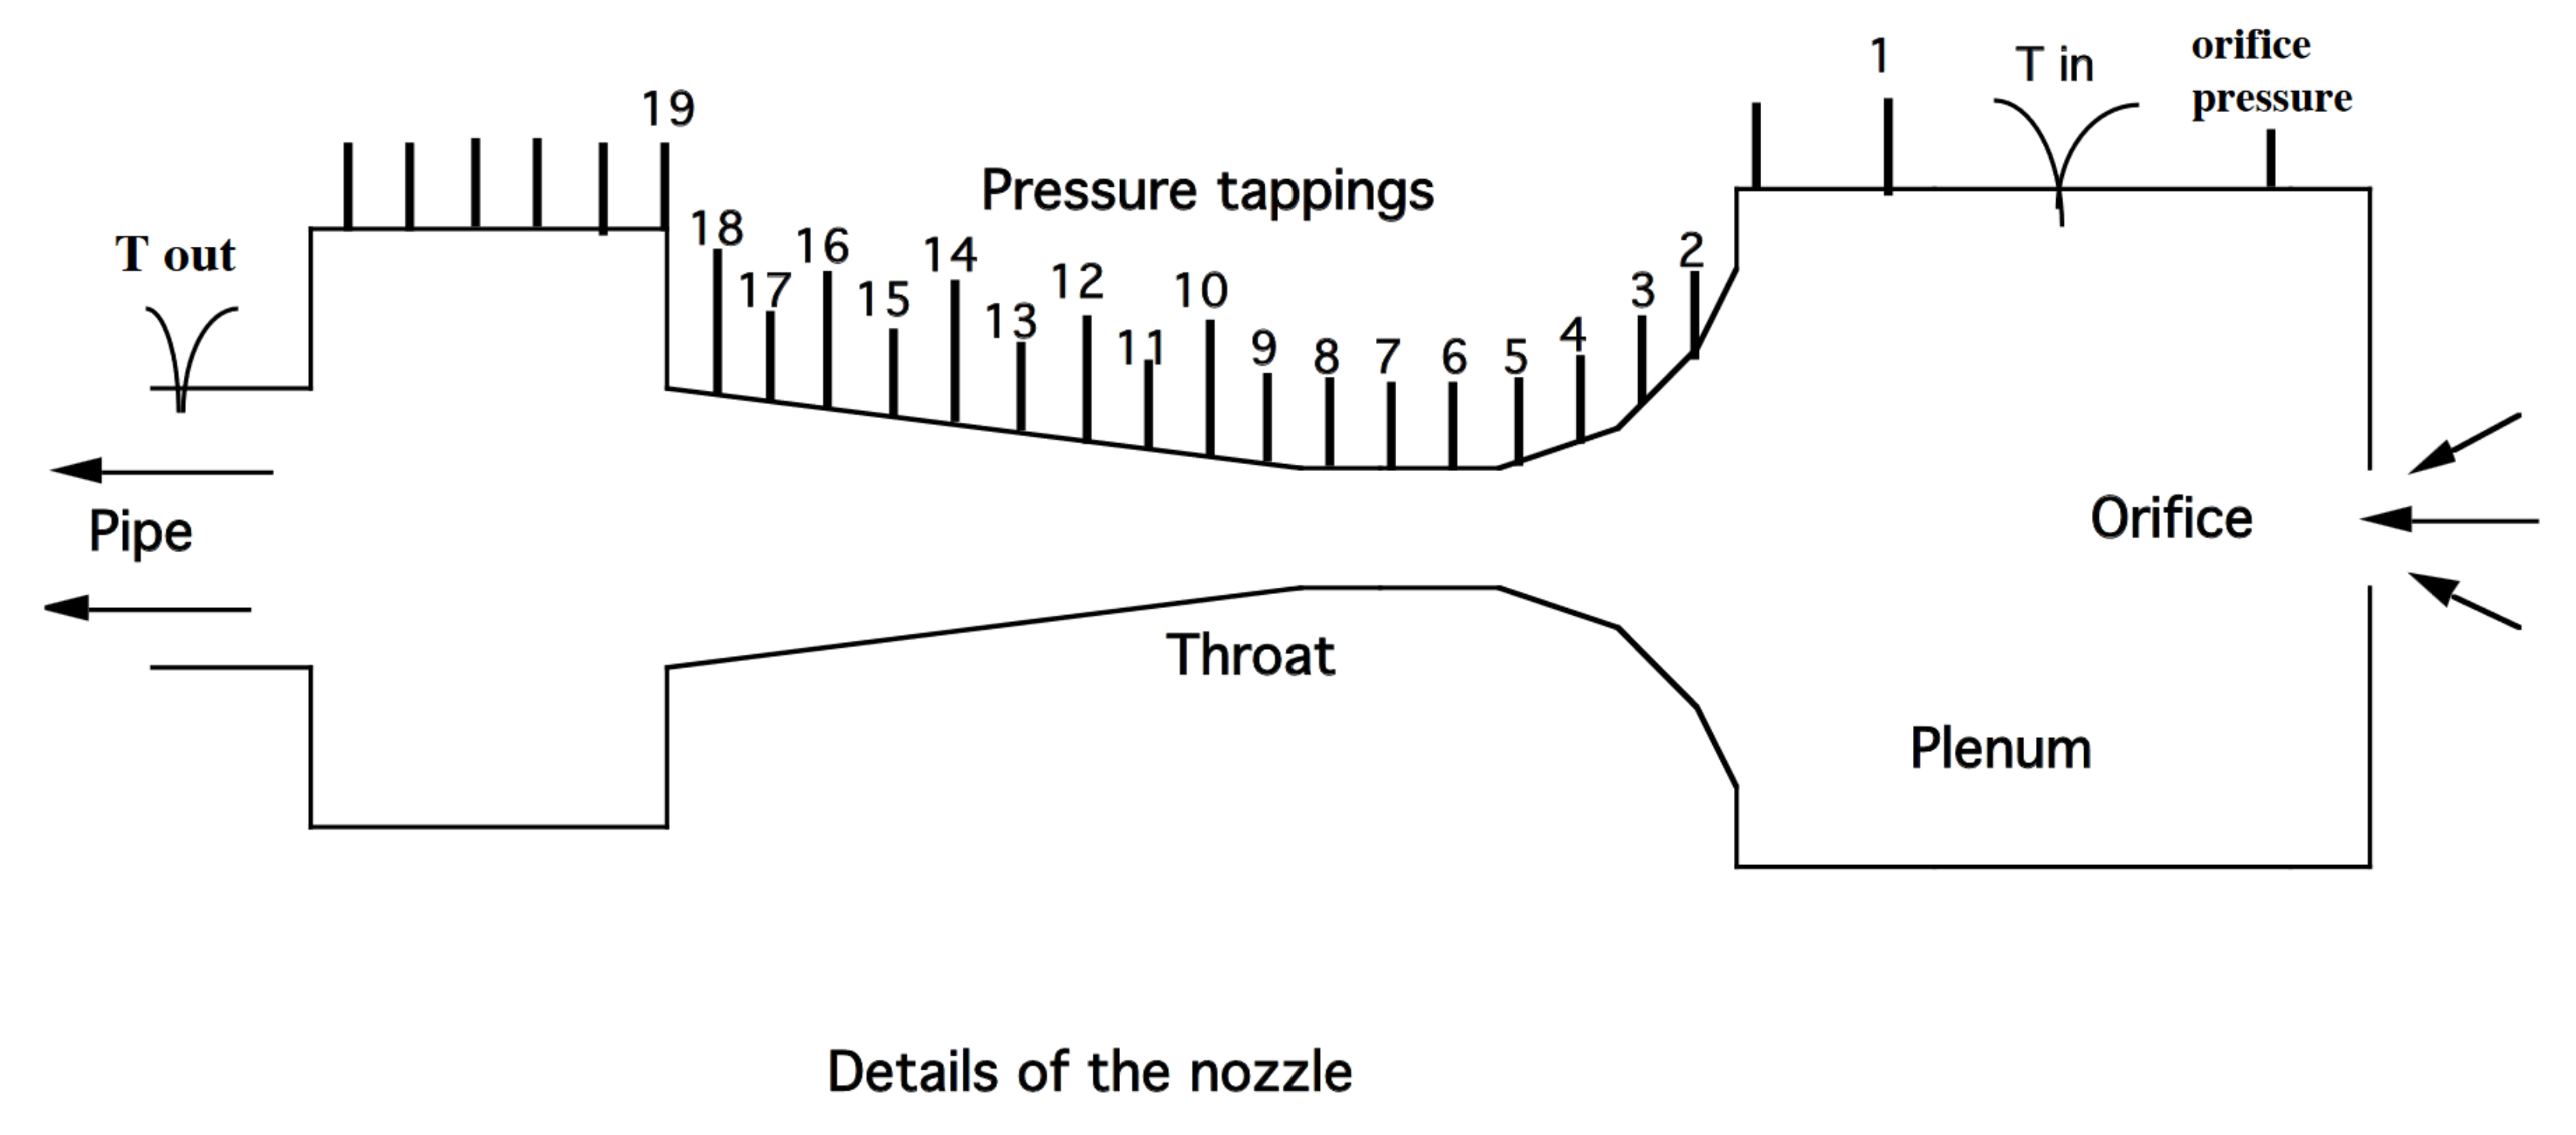
\includegraphics[width=0.8\textwidth]{small_nozzle_layout.png}
    \caption{Layout of Convergent - divergent nozzle}
    \label{fig:figure1}
\end{figure}

Orifice calibration: the diameter of the orifice is 17.47 mm. To a first approximation, assume that
\begin{itemize}
    \item The flow into the orifice is inviscid,
    \item the flow is slow enough to be treated as incompressible with density equal to that in the atmosphere upstream of the orifice (where the velocity is negligible),
    \item the velocity is uniform across the plane of the orifice,
    \item the pressure difference between the orifice plane and the upstream atmosphere is that measured on the
    water manometer
\end{itemize} 

The first assumption is valid, due to the thin section of the orifice. This means that up to and including the small oriface surface, the flow can be treated as inviscid, and Bernoulli's equation can be applied.
The second assumption requires further justification (in my eyes). The flow upstream of the oriface has a negligible velocity compared to that of the oriface, and so the density of the flow upstream of the oriface is equal to that of the atmosphere.
However, the flow through the oriface may be compressible due to the high velocity of the flow.
If we assume the nozzil is choked upstream of the oriface, then its non-dimensional mass flow rate is given by the following equation.
\begin{equation}
    \frac{\dot{m}\sqrt{c_pT_0}}{p_0A^*} = 1.281
\end{equation}
From this, the non dimensional mass flow rate at the oriface can be calculated using the area ratio of the oriface to the nozzle throat.
The area of the throat was not known however, but can be assumed to be at least less than half the area of the oriface.
At this area ratio of $0.5$, the density ratio $\rho/\rho_0$ is greater than $0.9535$, and so the assumption that the flow is incompressible is crude but sufficient for the purposes of this experiment.

\newpage


The third assumption that the velocity is uniform across the plane of the oriface is valid, as the oriface is thin and the flow is inviscid.

With these assumptions, the theoretical flow rate through the orifice can be calculated using the pressure difference between the orifice plane and the upstream atmosphere is that measured on the
water manometer. From applying the Bernoulli equation from the upstream atmosphere (1) to the oriface plane (2),

\begin{equation}
    p_1 = p_2 + \frac{1}{2} \rho_a v_2^2
\end{equation}

Where $A$ and $v_2$ are the cross-sectional area, and velocity at the oriface. The theoretical mass flow rate through the oriface is then given by the following equation.
\begin{equation}
    \dot{m} = \rho_a A v_2 = \rho_a \left( \frac{\pi D^2}{4}\right) \sqrt{\frac{2(p_1-p_2)}{\rho_a}} \;\;\;\;\;\; \text{where} \;\;\;\;\;\ p_2 - p_1 = \rho_w g \Delta h
\end{equation}
Where $\rho_a$ is the density of air and $\rho_w$ is the density of water used for the manometer.
However, the actual flow rate through the orifice differs from the theoretical value as our assumptions are not entirely valid.
This difference is characterised by the discharge coefficient $C_d$ which is defined as the ratio of the actual flow rate to the theoretical flow rate.
\begin{equation}
    \dot{m}_{actual} = C_d \dot{m}_{theoretical}
\end{equation}
% https://arc.aiaa.org/doi/pdf/10.2514/6.2019-3651 ?
The discharge coefficient of the oriface is effectively constant over the range of high reynolds numbers considered in this experiment. 

\begin{figure}[H]
    \centering
    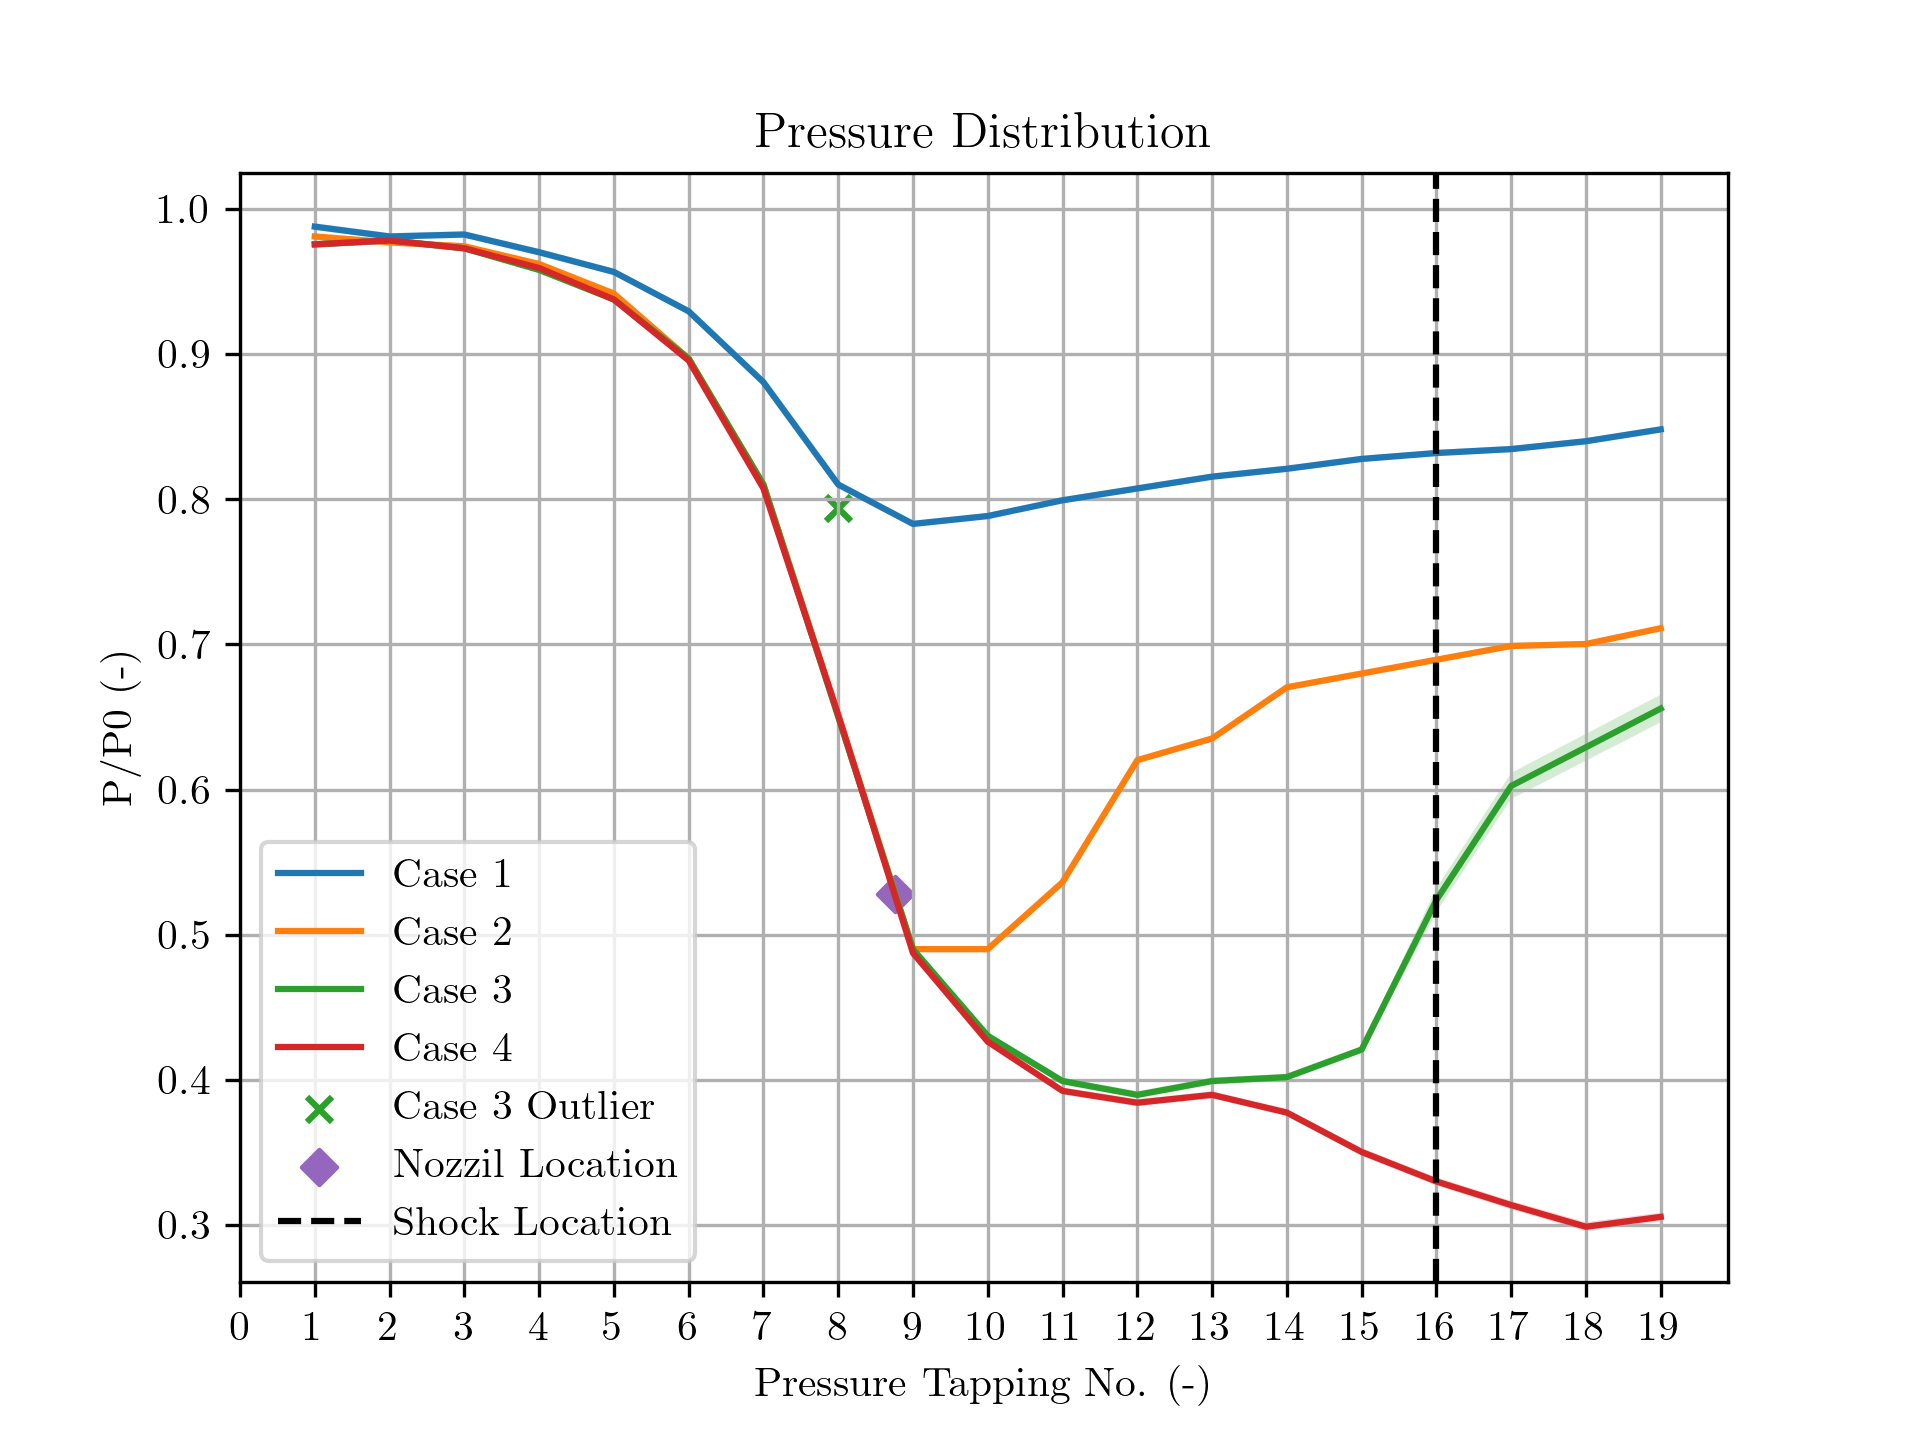
\includegraphics[width=0.8\textwidth]{pressure_ratio_distribution_corrected.png}
    \caption{Figure 1}
    \label{fig:figure4}
\end{figure}

\begin{figure}[H]
    \centering
    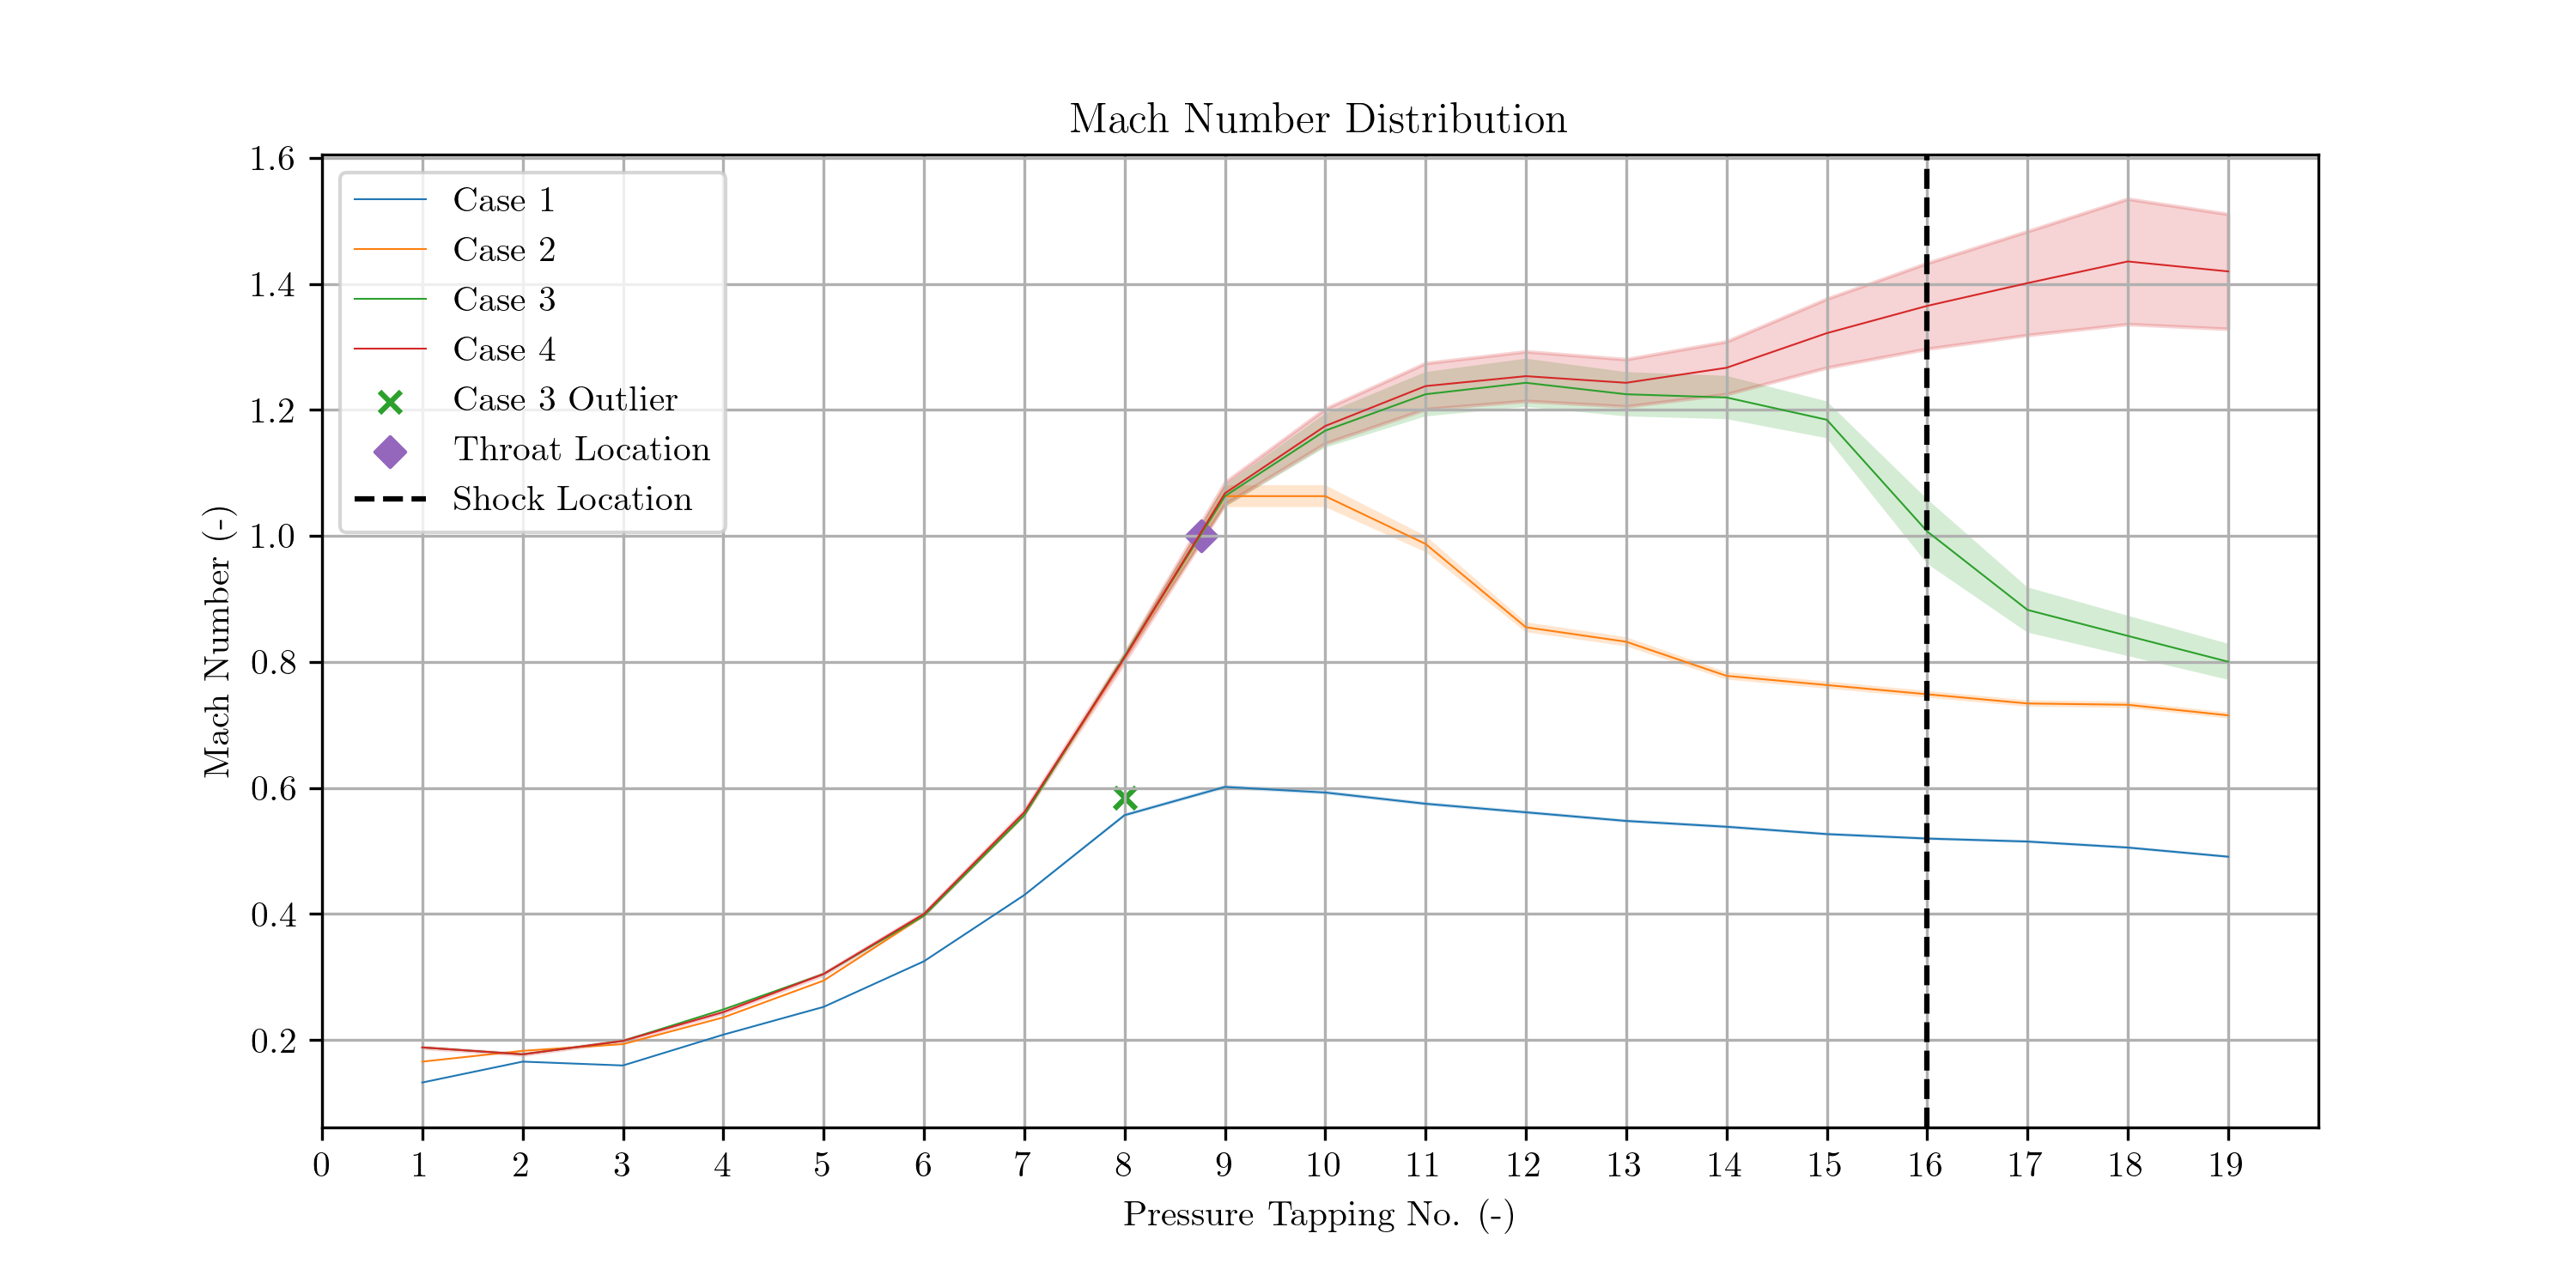
\includegraphics[width=0.8\textwidth]{mach_number_distribution_corrected.png}
    \caption{Figure 1}
    \label{fig:figure5}
\end{figure}


\begin{figure}[H]
    \centering
    \begin{subfigure}[t]{0.48\textwidth}
        \centering
        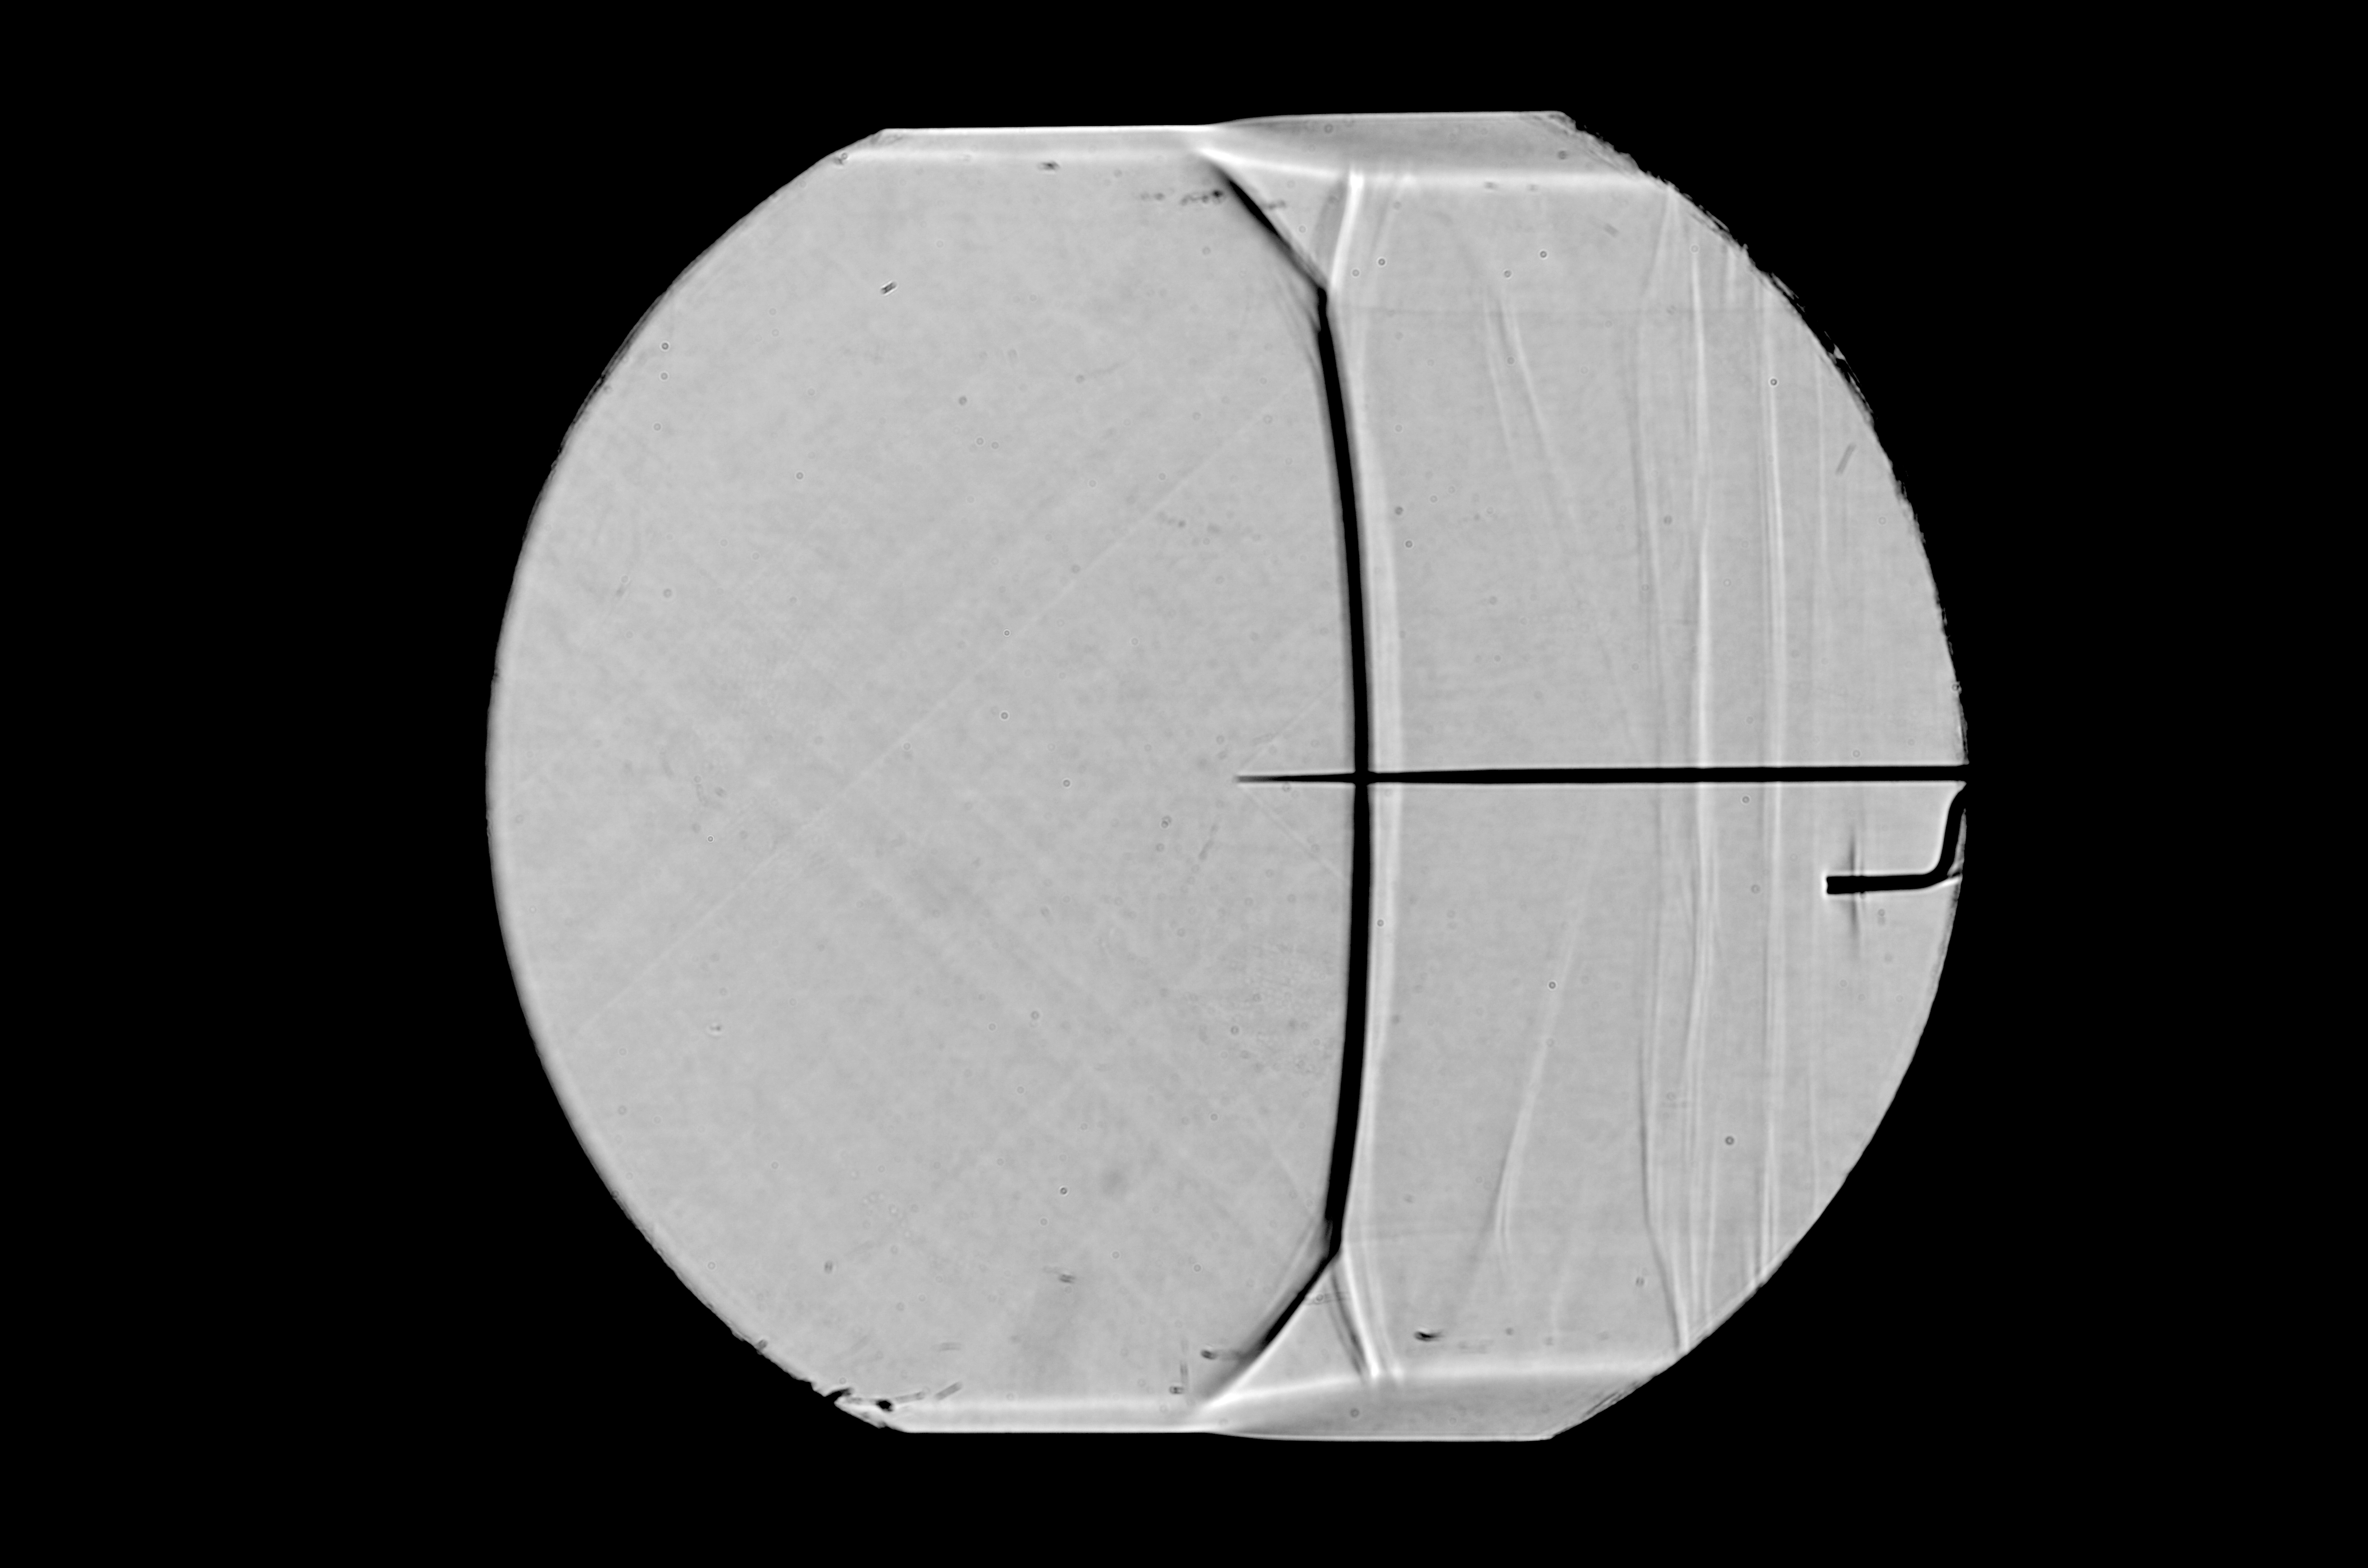
\includegraphics[width=1\textwidth]{starting_shock.jpg}
        \caption{Shock wave in working section before sensors}
        \label{fig:figure6}
    \end{subfigure}
    ~
    \begin{subfigure}[t]{0.48\textwidth}
        \centering
        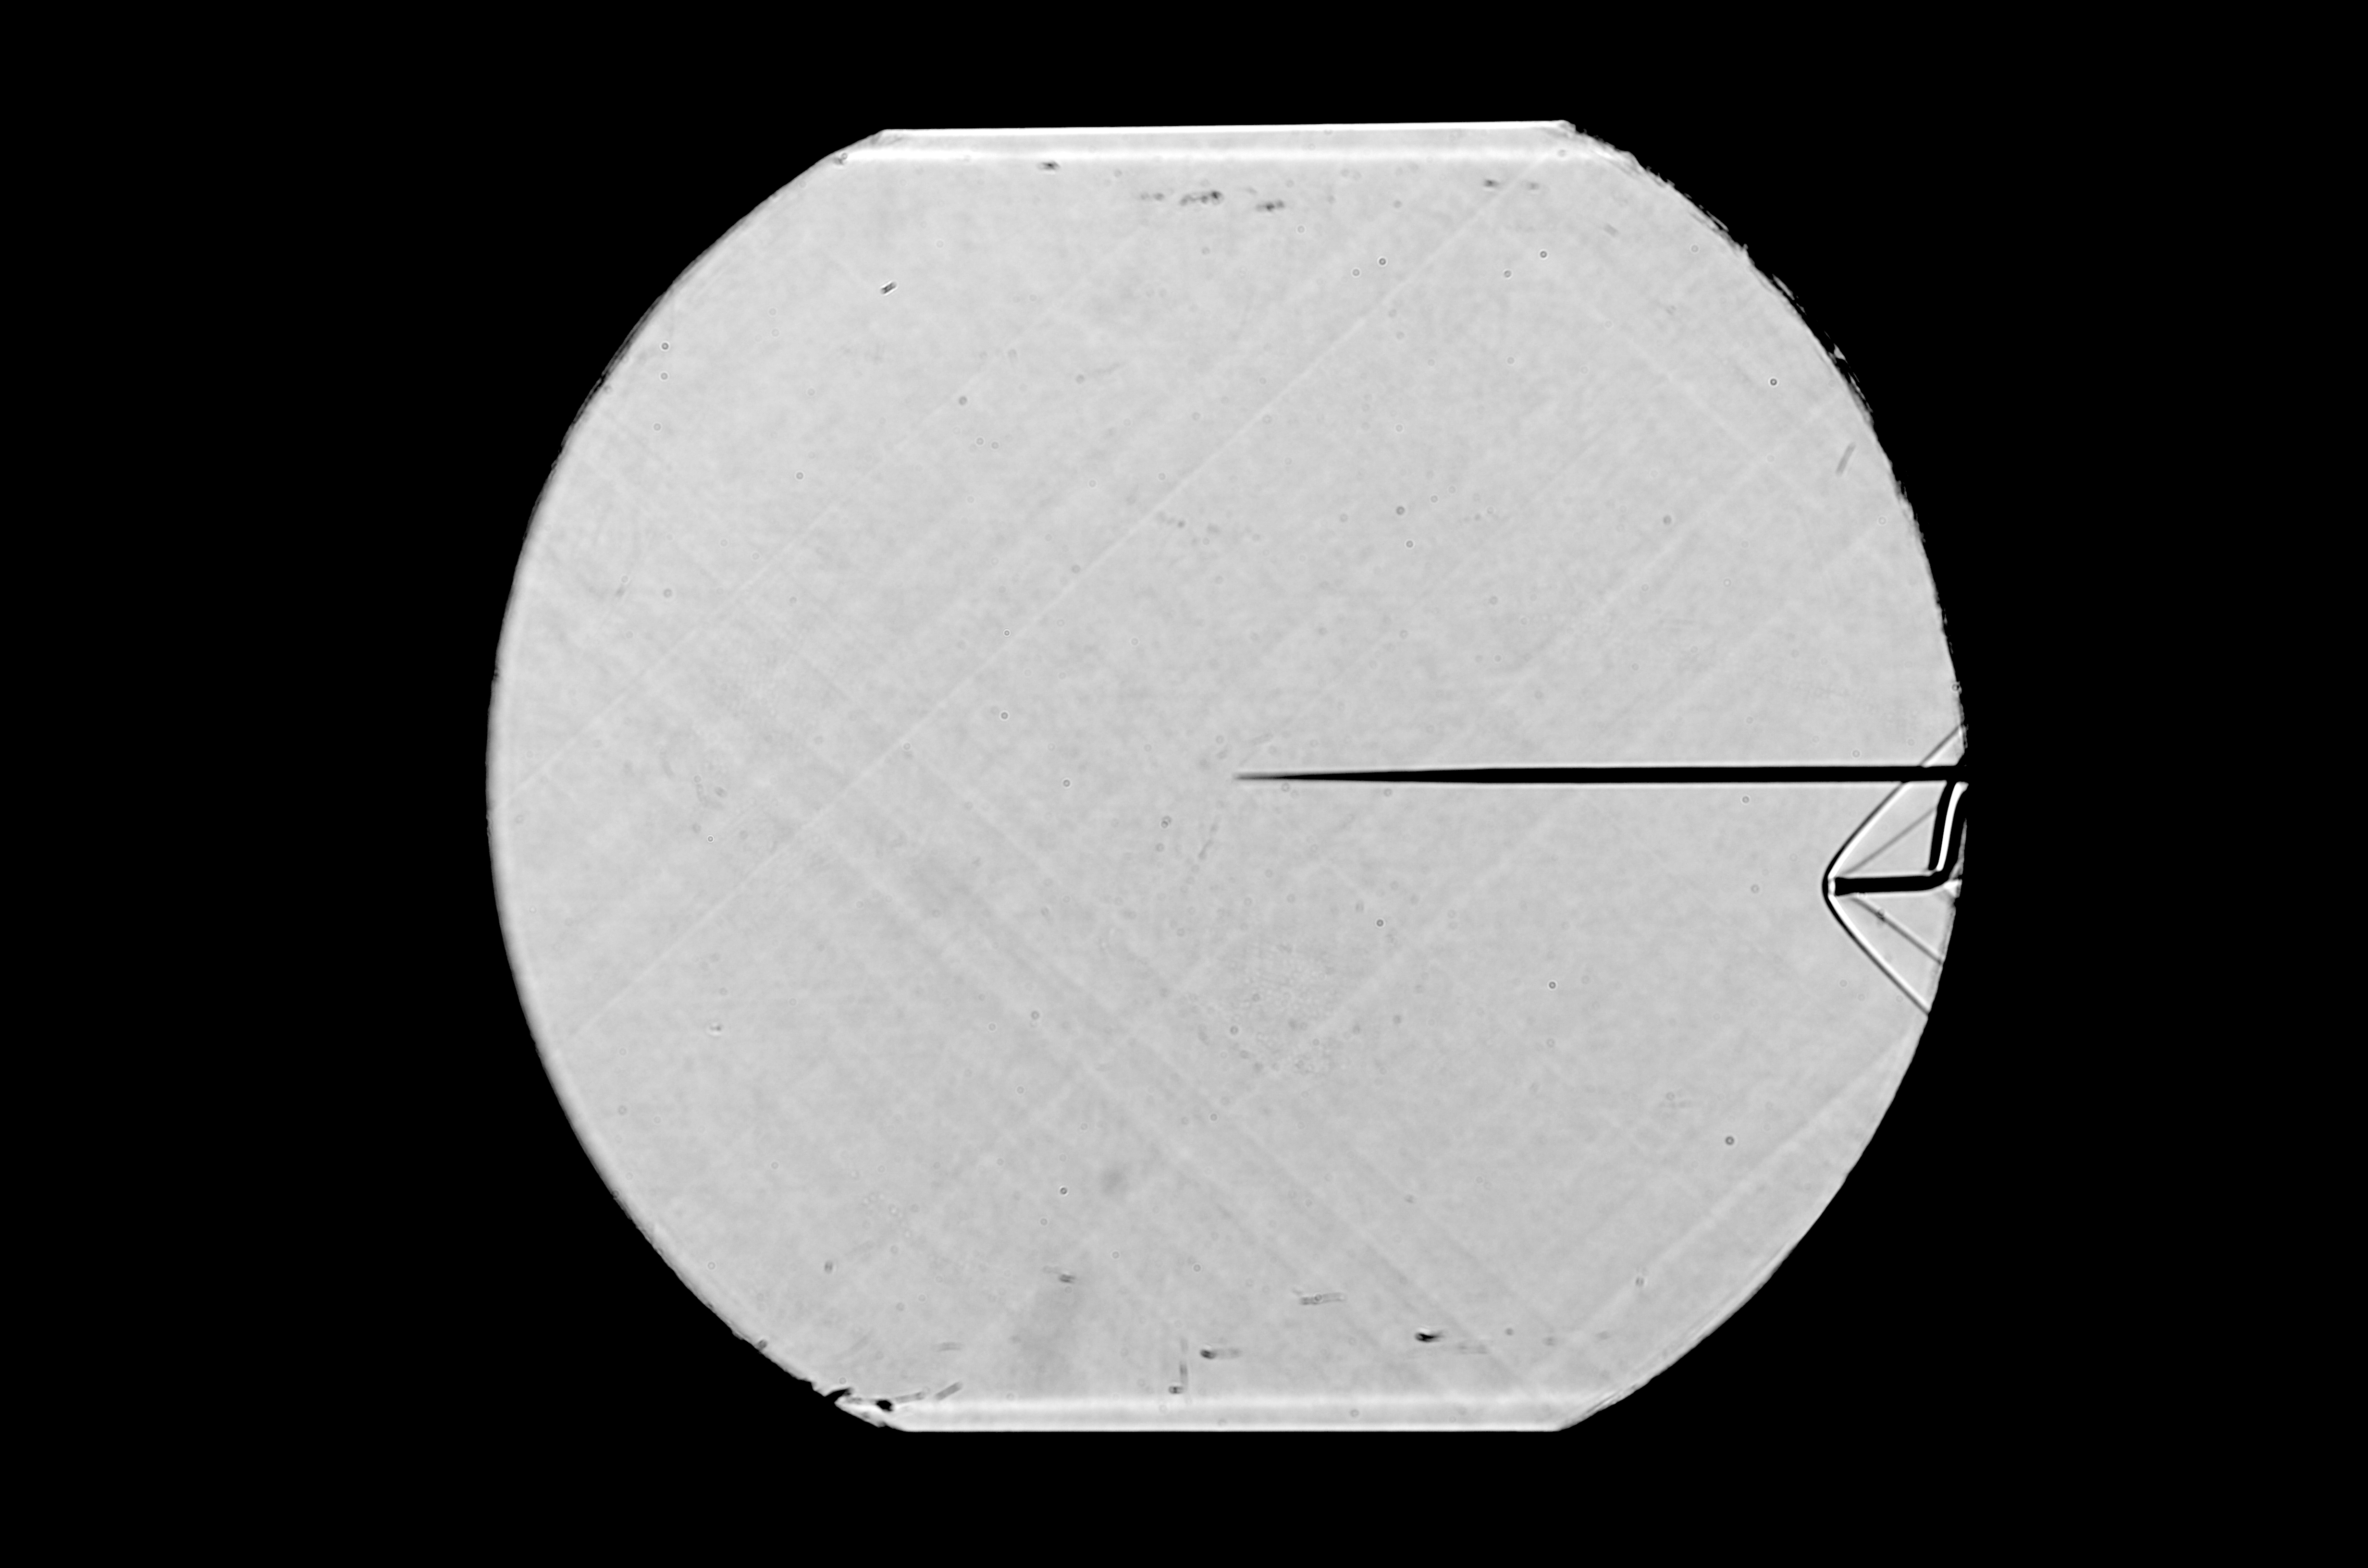
\includegraphics[width=1\textwidth]{working_state.jpg}
        \caption{Working state and bow shock of pitot probe}
        \label{fig:figure7}
    \end{subfigure}
    \caption{Shadowgraph images of the supersonic wind tunnel}
\end{figure}

Figure \ref{fig:figure6} shows the shock wave in the working section of the supersonic wind tunnel before the pressure sensors.
Shock waves of high density gradient are visible in the image from dark regions of the shadowgraph, where darker regions indicate stronger shock waves.
At the boundary layers at the top and bottom of the tunnel, the flow appears to travel through two shockwaves.
After the first shockwave the flow near the boundary layer is subsonic, but then must be accelerated again to supersonic speeds before the second, weaker shock.


\begin{figure}[H]
    \centering
    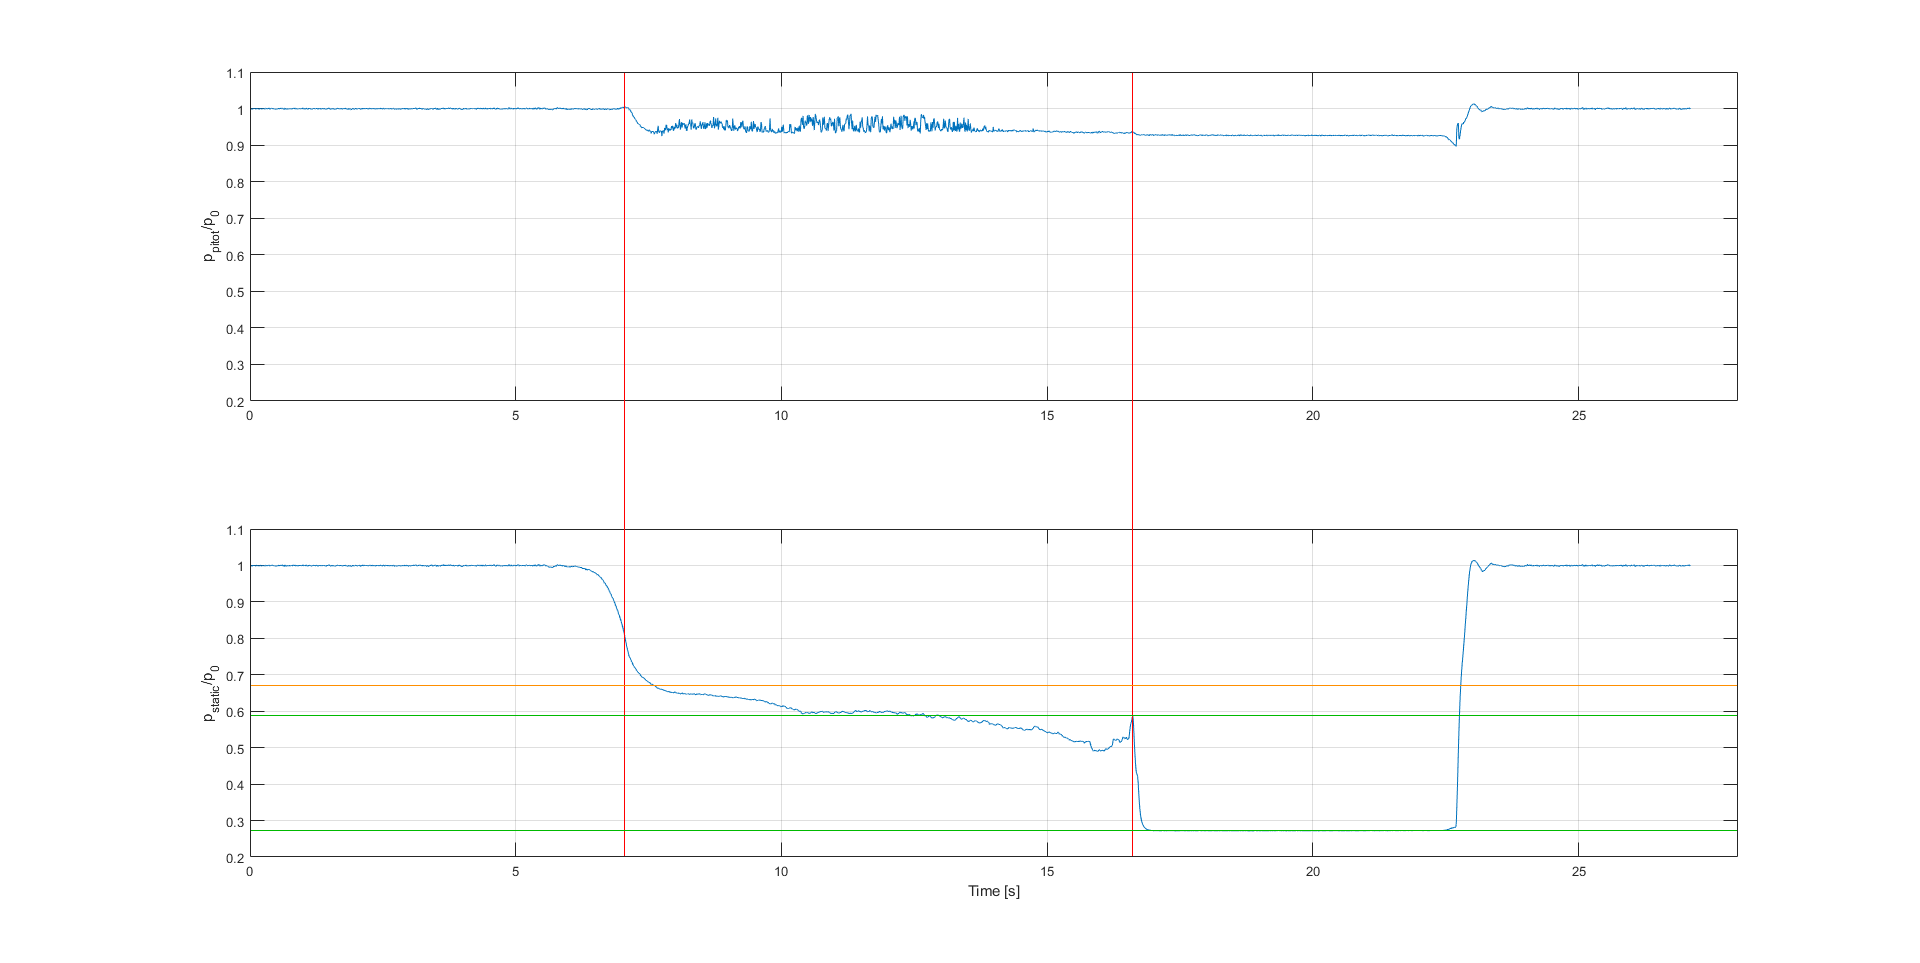
\includegraphics[width=1\textwidth]{tunnel_pressures_annotated.png}
    \caption{Annotated readings of the pressure sensors over time during the experiment. Top graph shows the stagnation pressure ratio, and the bottom graph shows the static pressure ratio.}
    \label{fig:figure8}
\end{figure}

Figure \ref{fig:figure8} shows the annotated readings of the pressure sensors over time during the experiment.
It can be observed that before the first vertical red line, the static pressure decreases which corresponds to the subsonic flow accelerating.
At the red line the normal shock wave is formed upstream of the sensors, by the supersonic flow downstream of the throat.
The stagnation pressure readings then becomes very noisy as the shock wave moves further downstream (WHY?) Shock trains?.
The static pressure ratio slowly decreases indicating an acceleration in the flow, and then suddenly increases again as the flow decelerates.


\newpage

\section{Discussion}

%interpret results and comment on anomalies

\subsection{Improvements}

\section{Conclusion}

From the experiments performed it can be observed that blah blah blah

\end{document}
